Il seguente codice MatLab, riguarda la funzione $\theta_{h}(x) = \frac{f(x+h)-f(x-h)}{2h}$, indicando con $h=10^-j$, $j=1,...,10$, $f(x)=x^4$ e $x=1$ :\\
\lstinputlisting[language=Matlab]{Cap_1/Es_3/Es_3.m}
restituisce i seguenti valori:\\
\begin{center}
\begin{tabular}{|c|c|}
\hline
h & \( \theta_{h}(1) \)  \\
\hline
    \(10^{-1}\) & 4.040000000000003e-02\\
    \(10^{-2}\) & 4.000400000000004e-04\\
    \(10^{-3}\) & 4.000003999999724e-06\\
    \(10^{-4}\) & 4.000000039999230e-08\\
    \(10^{-5}\) & 4.000000000403680e-10\\
    \(10^{-6}\) & 3.999999999948489e-12\\
    \(10^{-7}\) & 4.000000000115022e-14\\
    \(10^{-8}\) & 4.000000003445692e-16\\
    \(10^{-9}\) & 4.000000108916879e-18\\
    \(10^{-10}\) & 4.000000330961484e-20\\
\hline
\end{tabular}
\end{center} 
Si vede che i valori di $\theta_{h}(1)$ diminuiscono fino ad $h = 10^{-6}$, in cui si ha il minimo valore di $\theta_{h}(1)$, dopodichè l'errore inizia a crescere. Mostriamo l'andamento relativo nel seguente plot:
\begin{figure}[H]
\label{Cap_1_Es_3}
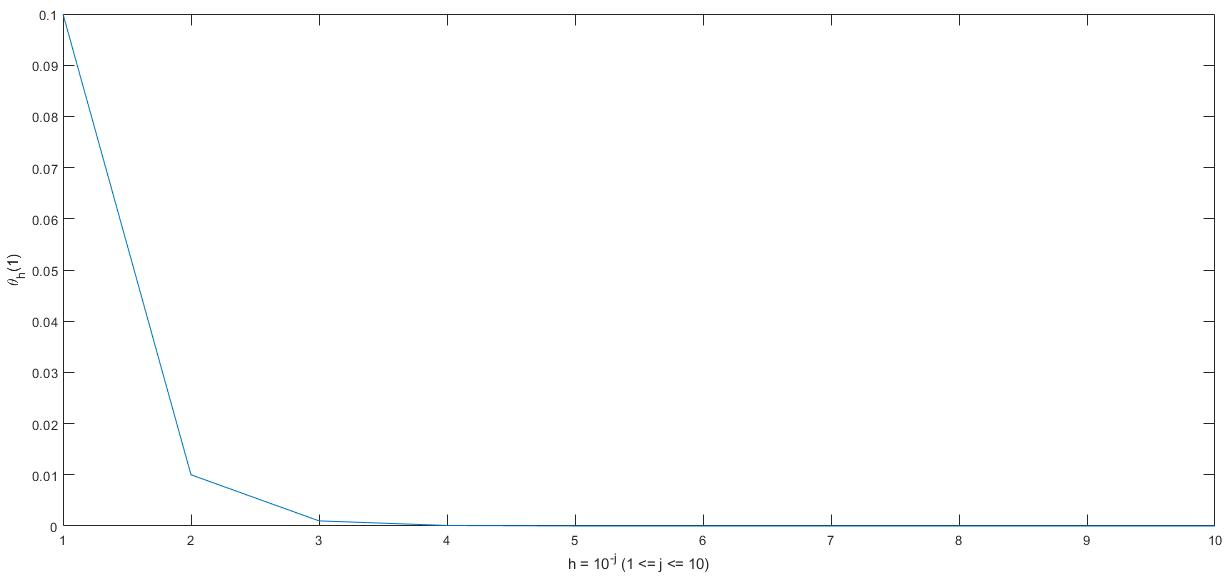
\includegraphics[left, width=150px]{Plot/Cap_1_Es_3}
\caption{Andamento della funzione $\theta_{h}(1)$}
\end{figure}